\section{Hypertex Transfer Protocol - HTTP/1.1}

Es el protocolo encargado de transferir \textbf{recursos} en internet. Los recursos son identificados por una \textbf{URI} (Uniform Resource Location). Las URIs tienen dos formatos: URN (Uniform Resource Name) o URL (Uniform Resource Location).

\begin{tcolorbox}[
    enhanced,
    colback=blue!3!white,         % Fondo celeste muy suave
    colframe=blue!60!black,       % Borde azul oscuro elegante
    title=\textbf{Funcionamiento de HTTP},
    fonttitle=\large\sffamily,    % Fuente del título sin serifas
    coltitle=white,
    boxrule=1.2pt,
    arc=6pt,                      % Bordes redondeados
    drop shadow=black!15!white,   % Sombra sutil
    left=10pt, right=10pt, top=10pt, bottom=10pt
]
Es un protocolo de solicitud/respuesta \textbf{sin estado}, de \textbf{texto plano}. Utiliza MIME para enviar datos binarios. Corre sobre \textbf{TCP puerto 80}. También existe una versión segura \textbf{HTTPS} que usa TLS; corre en \textbf{TCP puerto 443}. 

Cuando se solicita un recurso tenemos que esperar la respuesta, no hay un identificador que permita relacionarlas. Permite \emph{pipelining}.
\end{tcolorbox}

\subsection{Mensajes y Métodos}

\begin{enumerate}[label=\textcolor{acento}{\textbf{\arabic*.}}]
    \item Los clientes envían \textbf{request methods} al servidor mediante HTTP. Este request method indica al servidor qué acción ejecutar.
    \item El servidor ejecuta el method.
    \item El servidor responde con uno o más \textbf{response methods} que incluyen un código de estado, indicando si la solicitud fué exitosa o no, o si debe realizar alguna acción.
\end{enumerate}

Los mensajes tienen la misma estructura: línea de inicio, cabecera y cuerpo (opcional). 

\begin{figure}[H]
    \centering
    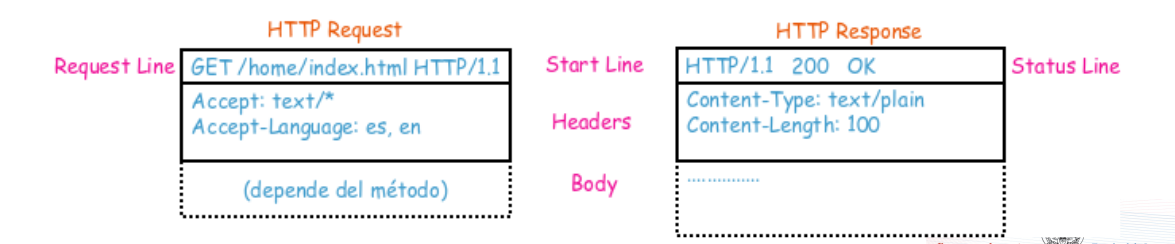
\includegraphics[width=0.8\textwidth]{capitulos/http1/imagenes/mensaje.png}
    \caption{Mensajes HTTP/1.1}
    \label{fig:http-mensaje}
\end{figure}

La \textbf{línea de inicio} es la primera de todos los mensajes HTTP, luego siguen las \textbf{cabeceras} de nombre-valor separadas por \texttt{:}, y por último el \textbf{body} que depende del método usado y del resultado de la operación. 

\subsubsection{Algunos Métodos}

Los métodos más utilizados son:

\begin{itemize}[label=\textcolor{acento}{$\bullet$}]
    \item \textbf{GET:} el cliente solicita un recurso al servidor. Podrían enviarse datos en el body, pero no es usual. Ejemplo: \texttt{http://www.example.com/index.php?pais=Argentina,deporte=tenis}. Los parámetros van después del \texttt{?}.
    \item \textbf{HEAD:} igual al GET pero solo se obtienen los \textbf{metadatos} del recurso (headers). No se envía el recurso solicitado.  
    \item \textbf{POST:} envía datos de entrada al servidor, que se mandan en el body. Solicita una respuesta del servidor.
    \item \textbf{PUT:} envía contenido que será almacenado en el webserver. 
    \item \textbf{DELETE:} indica contenido a ser eliminado del webserver.  
\end{itemize}

\subsection{Funcionamiento}

Cada mensaje puede tener ninguna o muchas cabeceras que agregan información adicional a los mensajes. Algunas cabeceras son:

\begin{itemize}[label=\textcolor{acento!60}{$\bullet$}]
    \item \textbf{Host:} obligatoria, infica el servidor y puerto destino.
    \item \textbf{Date:} día y hora de creación del mensaje.
    \item \textbf{Content-Lenght:} longitud del cuerpo del mensaje.
    \item \textbf{Content-Type:} tipo de objeto que se envía.
\end{itemize}

\begin{figure}[H]
    \centering
    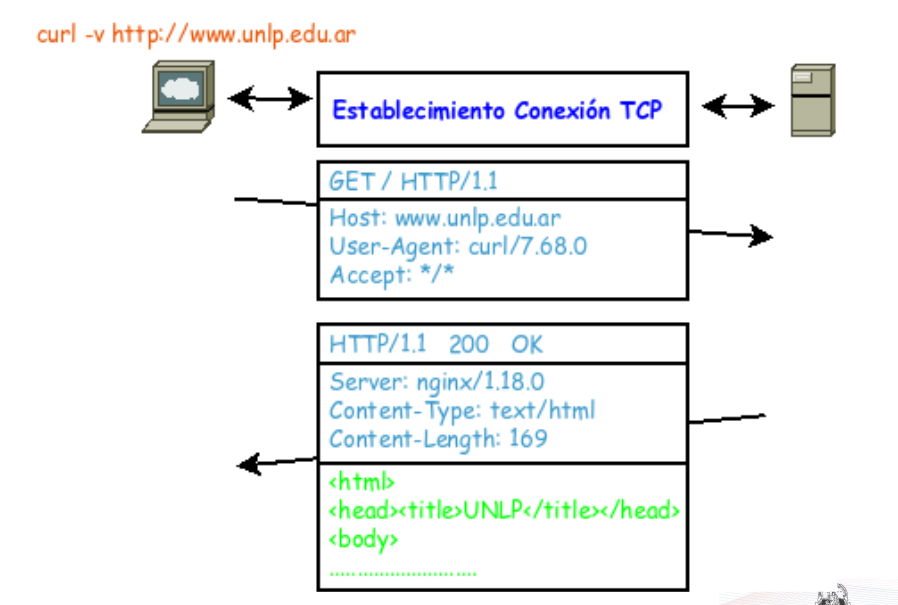
\includegraphics[width=0.8\textwidth]{capitulos/http1/imagenes/funcionamiento.png}
    \caption{Funcionamiento de HTTP/1.1}
    \label{fig:http-funcionamiento}
\end{figure}

\begin{nota}{\emph{\textbf{Recordar...}}\smallskip}
    En \textbf{HTTP/1.0} las conexiones eran \textbf{no persistentes}, es decir, se transfiere un objeto por cada sesión y por cada recurso se debe abrir y cerrar una sesión TCP. El servidor responde con un objeto y cierra la sesión (algunas implementaciones de HTTP/1.0 soportan conexiones keep-alive, pero no es lo default).
\end{nota}

En HTTP/1.1 las conexiones son \textbf{persistentes por defecto}, y con las cabeceras \emph{Connection: close} indicamos que queremos cerrar la conexión después de la respuesta del server. 

\begin{figure}[H]
    \centering
    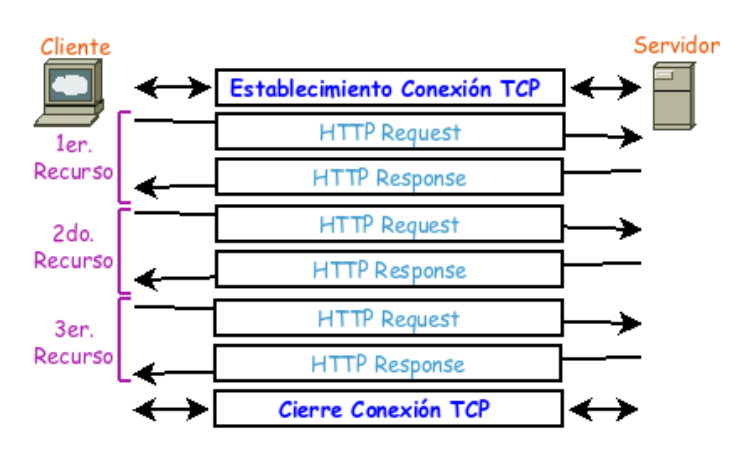
\includegraphics[width=0.8\textwidth]{capitulos/http1/imagenes/conexiones-persistentes.png}
    \caption{Conexiones persistentes de HTTP/1.1}
    \label{fig:http-conexiones-persistentes}
\end{figure}

\begin{definicion}{Concurrencia en HTTP/1.1}
    Este protocolo permite \textbf{pipelining:} el cliente puede enviar muchas solicitudes sin esperar cada respuesta, y el servidor las procesa en paralelo. Tiene que enviar las respuestas en el \textbf{mismo orden} que recibió las solicitudes.
    
    Los clientes pueden abrir \textbf{conexiones simultáneas} a un servidor, usadas para evitar el \emph{head-of-line blocking}.    
\end{definicion}

Se puede hacer un \textbf{GET Condicional} con la cabecera \texttt{If\_Modified\_Since}, donde el servidor retorna el recurso si fué modificado en una fecha posterior a la indicada en el header. Si no fue modificada, se responde con código \texttt{304} y el recurso se recupera de caché.

Si el recurso fué designado a una nueva URL, el server responde con \texttt{301 (Moved Permanently)} o \texttt{302 (Found)}, y agrega una cabecera \texttt{Location} con la nueva URL.

\subsection{HTTPS}

Es HTTP con TLS, sobre TCP en puerto 443. Los mensajes HTTP se \textbf{encriptan y autentican de forma completa}. 

\begin{figure}[H]
    \centering
    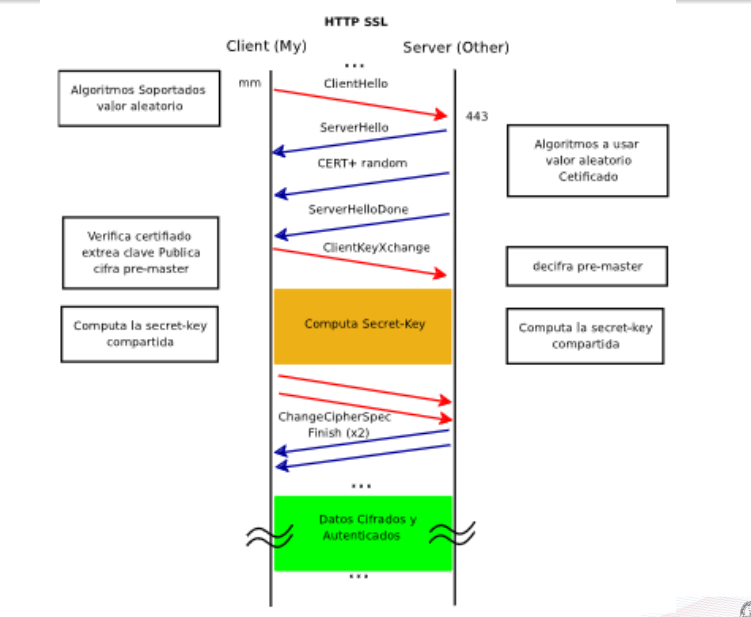
\includegraphics[width=0.8\textwidth]{capitulos/http1/imagenes/https.png}
    \caption{TLS en HTTP/1.1 (HTTPS)}
    \label{fig:http-https}
\end{figure}

\subsection{Cookies}

Las cookies permiten a las aplicaciones web del server \textbf{manejar estados} conservando información entre peticiones del cliente, ya que HTTP/1.1 no maneja estados por defecto. 

Los servers envían información de estado con un header \texttt{Set-Cookie}, y en las siguientes solicitudes el cliente retorna una cabecera \texttt{Cookie} con los datos recibidos.

\begin{figure}[H]
    \centering
    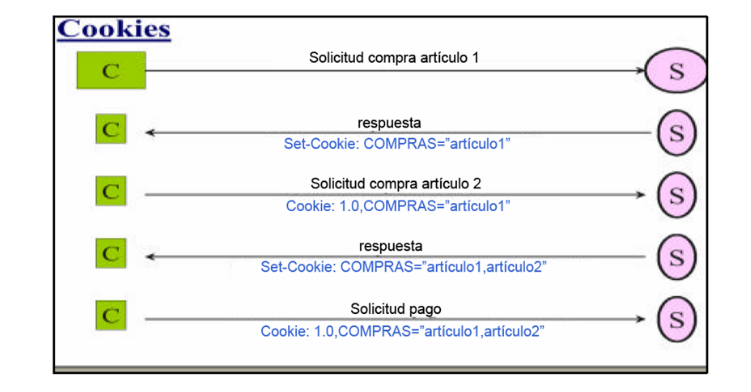
\includegraphics[width=0.6\textwidth]{capitulos/http1/imagenes/cookies.png}
    \caption{Ejemplo de uso de Cookies}
    \label{fig:http-cookies}
\end{figure}

\subsection{Caching}

Es una característica opcional de HTTP/1.1 que consiste en almacenar de forma local los mensajes de respuesta para reducir el tiempo de respuesta y carga de la red. 

Hay que asegurar que los contenidos guardados en caché sean equivalentes a los almacenados en el servidor, generalmente almacenan respuestas exitosas de una solicitud de recuperación. 

Si la solicitud es servida desde cache se conoce como \textbf{cache hit}, y si no se encuentra en la cache es un \textbf{cache miss} y se pide el recurso al webserver. Cuando el recurso está en la caché pero no es válido, se tiene que revalidar utilizando un \texttt{GET} condicional. 